
\documentclass[runningheads,a4paper]{llncs}

\usepackage{amssymb}
\setcounter{tocdepth}{3}
\usepackage{graphicx}

\usepackage{url}
\urldef{\mailsa}\path|dejun@cs.pdx.edu|
\newcommand{\keywords}[1]{\par\addvspace\baselineskip
\noindent\keywordname\enspace\ignorespaces#1}

\begin{document}

\mainmatter  % start of an individual contribution

% first the title is needed
\title{coDoc: A Tool for Managing Relationships between Code and Documentation}

% a short form should be given in case it is too long for the running head
\titlerunning{coDoc: Managing Relationships between Code and Documentation}

% the name(s) of the author(s) follow(s) next
%
% NB: Chinese authors should write their first names(s) in front of
% their surnames. This ensures that the names appear correctly in
% the running heads and the author index.
%
\author{Dejun Qian}
%
\authorrunning{coDoc: Managing Relationships between Code and Documentation}
% (feature abused for this document to repeat the title also on left hand pages)

% the affiliations are given next; don't give your e-mail address
% unless you accept that it will be published
\institute{Computer Science Department,\\
Portland State University,\\
1900 SW 4th Avenue Portland, OR 97201, USA\\
\mailsa\\
\url{http://www.pdx.edu/computer-science/}}

%
% NB: a more complex sample for affiliations and the mapping to the
% corresponding authors can be found in the file "llncs.dem"
% (search for the string "\mainmatter" where a contribution starts).
% "llncs.dem" accompanies the document class "llncs.cls".
%

\toctitle{Lecture Notes in Computer Science}
\tocauthor{Authors' Instructions}
\maketitle


\begin{abstract}
The reuse of either software or hardware components is an important way to build large systems.
Documentation plays a critical role in the process of reusing,
as it describes how the components can be reused.
When writing and testing software, 
we need the documentation in hand.
This is particularly true for software that is documentation-intensive, 
such as device drivers and virtual device modules.
This paper presents coDoc, 
an integrated development environment for managing relationships between code and documentation.
We describe the architecture and features of coDoc,
and discuss several design decisions that we faced in developing coDoc and the trade-offs involved in making these decisions.
We report our experiences in mapping two virtual network interface card (NIC) modules to the real NIC documents by coDoc.
\keywords{Software Engineering, Data Model}
\end{abstract}


\section{Introduction}
\label{sec:introduction}
Documentation plays an important role in software engineering.
%from requirement analysis to architecture design,
%from coding to software testing,
%from software debugging to software maintenance.
Software that relates closely to hardware is extremely documentation intensive. % explain why
Examples of such software include bootloaders, 
Hardware Abstraction Layers (HAL) in Operating Systems (OS),
and virtual device modules for virtual machines.
Such software must follow the hardware documentation to operate correctly.
A typical embedded CPU might have documentation consisting of thousands of pages.
A computer system usually consists of more than ten hardware modules.
Effectively maintaining the relationships between the code and the documentation is important for developing and verifying hardware-related software.

To our knowledge, there are no tools to address this problem.
Researchers have done a lot of work to handle the relationships between Application Programming Interface (API) documents and their client code \cite{Pandita_inferring_2012} \cite{wei_inferring_2011}.
However, the approaches developed in the work do not consider the relationships between hardware-related code and its documentation.
API documents are usually well indexed by the functions or the classes that they define.
When we are interested in a piece of code in the client software
we can easily find the related API documents by the names of the functions that the piece of code calls.
% The relationships between the client codes and the API documents can be easily constructed by using the function names as the keywords.
However, the code relating to hardware and its documentation usually relate in different ways.
% the hardware docuemnts are not orgnized by functions or classes, which are the basic elements of code, but instead by hardware modules.
People usually organize hardware documentation by hardware modules and the registers inside the hardware modules.
These modules and registers do not relate to the code in an explicit way.
Hardware documents include text, tables and diagrams, while API documents usually include text only.

% These differences make the constructing of the relationships between the hardware related codes and their documents really challenging.
A simple workaround is to include references to the positions of the related documentation as comments in the code.
However, this can only handle simple situations.
If there are thousands of such comments cluttered in the code,
it will be very hard to manage them.

This paper presents coDoc, a tool to create, maintain, and display relationships between code and documentation.
% The initial version\footnote{\texttt{\url{git@github.com:derekqian/coDoc.git}}} has been released.
The key features of coDoc include 
the ability to display both code and documents, 
the ability to write and edit code, 
code-piece selection based on syntax tree of the code,
%stable code selections regarding to the changes of unrelated codes;
creation of relationships between codes and documents,
and relationships management and display.
Using coDoc, we have created relationships between two virtual NIC devices in QEMU and the related documents.
These two devices are DIO \cite{dio} and E100 \cite{e100}.

The main contributions of this paper are as follows.
\begin{itemize}
\item Design a framework to display and manage codes, documents and relationships.
\item Design coDoc which implement the framework.
\item Maintain integrity of the relationships when the code evolves.
\item Design a standard format to represent the code piece.
\item Design a standard format to represent the document piece.
\item Design a data model for relationships between code and documentation.
\end{itemize}

The rest of the paper is organized as follows. 
Section \ref{sec:arch} provides the overall architecture and key features of coDoc.
%Section \ref{sec:decision} gives the design decisions of coDoc and the trade-offs of these decisions.
Section \ref{sec:evaluation} summarizes our experiences of creating and maitaining the relationships for two virtual devices.
Section \ref{sec:related} presents the related work.
Section \ref{sec:conclusion} concludes our work and gives our future research plan.

\section{Architecture and Features of coDoc}
\label{sec:arch}

\begin{figure}
\begin{center}
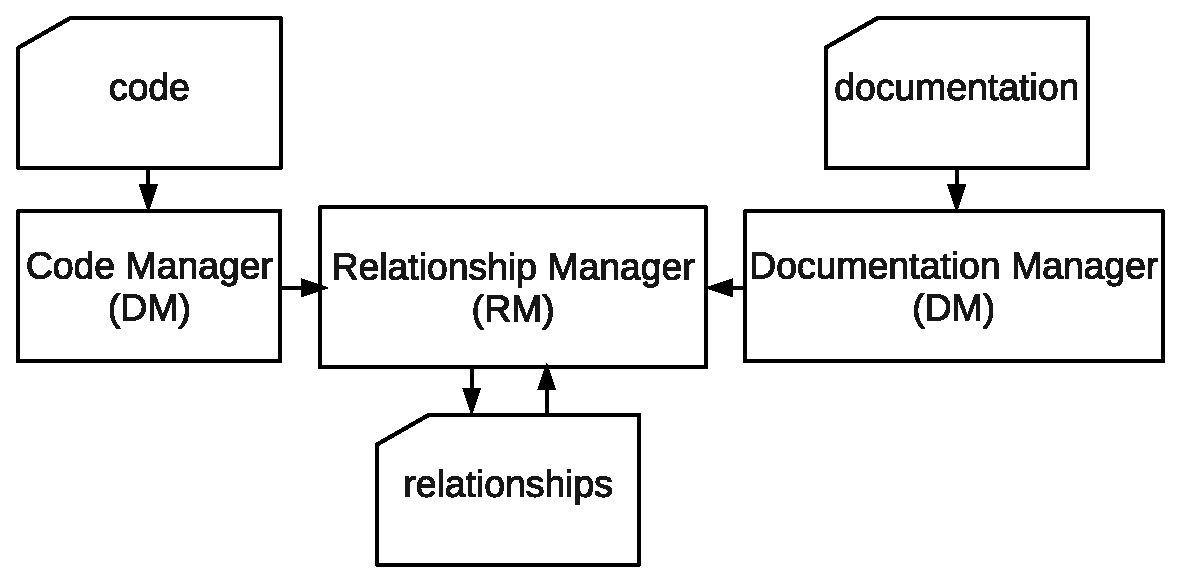
\includegraphics[width=0.55\textwidth]{architecture}
\caption{coDoc Architecture and Features}
\label{fig:architecture}
\end{center}
\end{figure}

\subsection{Architecture of coDoc}
The architecture of coDoc is shown in Figure \ref{fig:architecture}. 
It contains a code manager (CM), a documentation manager (DM) and a relationship manager (RM).
There are three types of data here, 1) code, 2) documentation, and 3) relationships.
We handle only C/C++ code at this time, 
as most system code is written in C/C++.
CM reuses C/C++ Development Tool (CDT) editor from Elipse\footnote{\texttt{\url{http://www.eclipse.org}}} to handle C/C++ code.
The CDT editor reads and parses the code, 
and highlights syntax elements.
We use poppler to read the PDF file and render the PDF pages as images.
As poppler is developed in C++ and Eclipse Rich Client Program (RCP) is in Java,
we need an adaptor to bridge between C++ and Java,
for which we use Java Native Interface (JNI).
We implement this adaptor in PDF Editor, 
and uses it to get the PDF page from poppler and display the page.
RM reads the relationship data,
and highlights the code and document pieces that are related.


\begin{figure}
\begin{center}
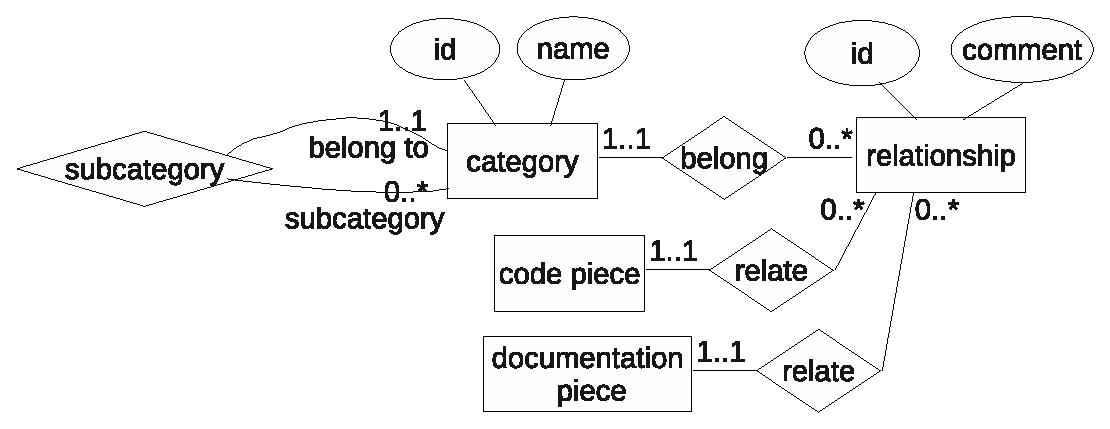
\includegraphics[width=0.85\textwidth]{datamodel}
\caption{Data Model for coDoc}
\label{fig:datamodel}
\end{center}
\end{figure}

\subsection{Data Model}
The data model is shown in Figure \ref{fig:datamodel}.
We have four entities here: category, relationship, code piece and documentation piece.
Code piece and documentation piece represent the selected code and documentation respectively.
We represent the relationships between code and documentation as entities,
as we want to classify the relationships.
The relationships are classified by their functionality in our approach.
Category is used to maintain the classification information of the relationships.
To represent a relationship, 
we need to define the strategy to represent the code piece and documentation piece.


\begin{figure}
\begin{center}
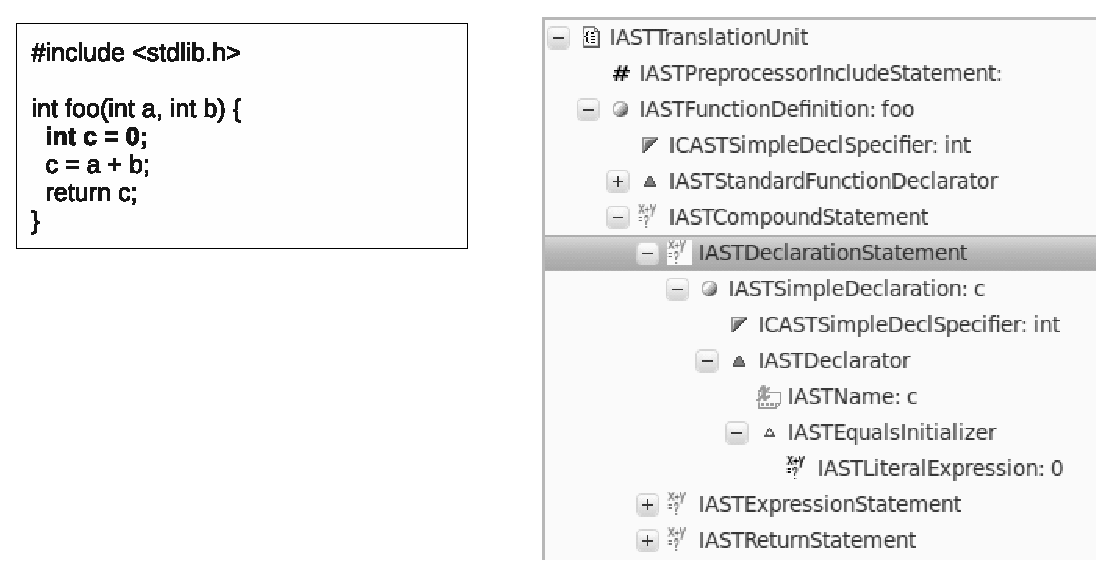
\includegraphics[width=0.85\textwidth]{ast1}
\caption{Original code and its AST}
\label{fig:ast1}
\end{center}
\end{figure}

\begin{figure}
\begin{center}
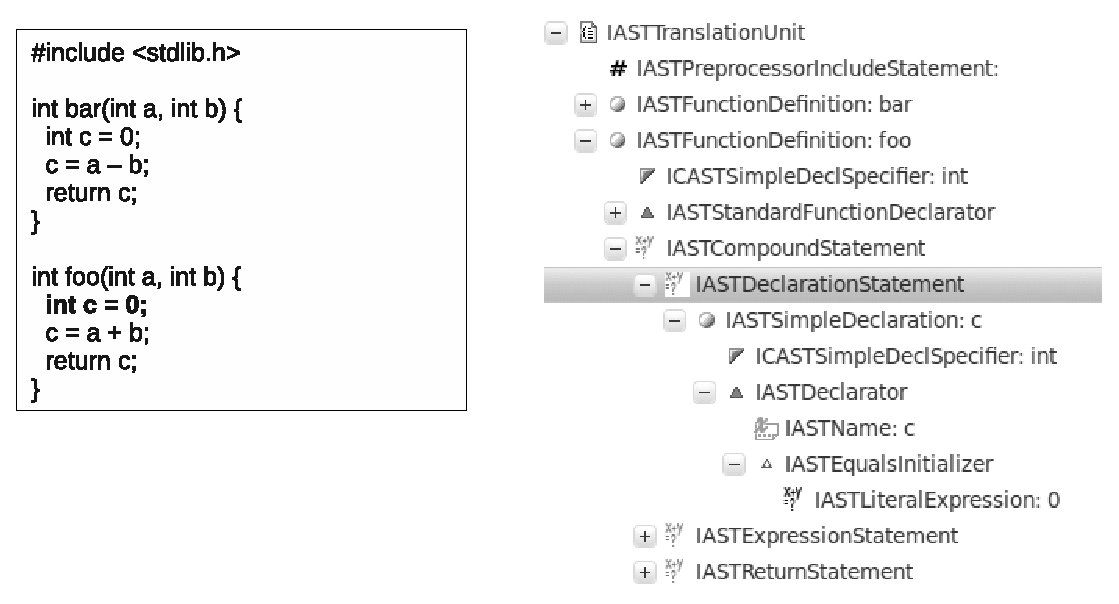
\includegraphics[width=0.85\textwidth]{ast2}
\caption{Evolved code and its AST}
\label{fig:ast2}
\end{center}
\end{figure}

\subsection{Representing Code Segments}
Code is always evolving during its lifetime.
We want the relationships created for one version of code keep working for other versions.
To achieve this goal, we need a robust strategy to represent the code pieces.
Our first method represents the code piece by the offset of the selected code from the beginning of the code file and the length of the selected code.
This method is straight forward and is easy to understand and implement.
However, this method is not robust,
as the change of the code file will change the offset of the selected code.
The left sides of Figure \ref{fig:ast1} and Figure \ref{fig:ast2} give the code before and after it evloves.
The highlighted code piece is what we want to select.
Unfortunitely, the offset of the select code increases after we add some code,
as shown in this example.
To achieve robustness, we need to find some properties of the code that are relatively stable when code evolves.
These properties can serve as keys to represent the code piece.
An intuitive thought is to use the semantic information,
that is the intrinsic meaning of the code.
However, we can't find a formal way of defining this information.
We use syntax information to form the main element of our code piece identifier.
The code can be parsed and represented by a syntax tree.
A change of the code in one branch will usually not affect the code in other branches.
Representing code segments based on the position in the syntax tree should be robust.
The right sides of Figure \ref{fig:ast1} and Figure \ref{fig:ast2} are the Abstract Syntax Trees (AST) for the code before and after it evolves.
In the ASTs, the highlighted nodes relate to the code piece we selected.
Through the two ASTs are different, 
the highlighted nodes can be represented by the same path from the roots of these two ASTs.
%To make the method more robust, % prof lost here
%we can introduce the information in the first method as the secondary key.
%When the syntax identifier fails to locate the code piece,
%we can use the offset information to assist the decision.
%We also include in the identifier the content of the code piece as an integrity check.
%The structure used to achieve this goal is shown bellow.
%\begin{Verbatim}[frame=single]
%class CodeSelection {
%  private String syntaxcodepath;
%  private String selcodepath;
%  private String syntaxcodetext;
%  private String selcodetext;
%}
%\end{Verbatim}


%\section{Methodology and Design Decisions}
%\label{sec:decision}
%\subsection{Embedded vs Seperate for PDF Reader}
%The tool should display both codes and documents at the same time.
%We can implement the code viewer and the PDF viewer in seperate process,
%and use inter process communication (IPC) techniques to communicate.
%The advantage of this method is that each process has its own window,
%can occupy the whole screen,
%and display more content which reduces the need to scroll the window horizontally.
%When the user uses a computer with two monitors,
%the tool implementing this method is an extremely good choice,
%as the user can choose to display the code and the document on seperate moniters.
%However, this implementation is heavy, % ?
%and has performance issues.
%When using the tool, 
%the user may need to launch the PDF reader,
%which is slow.
%Our earlest implementation uses this method,
%and encountered synchronization problems from the IPC communication.
%In coDoc, we choose to implement the code viewer and the PDF viewer in the same process.
%%The Eclipse framework even makes the whole system single thread.
%This way, all the commucation is internal to the same process,
%No IPC communication is needed,
%which is more efficient and makes the tool more responsive.
%With the new method, we can smoothly operate the tool without any uncomfortable feeling.
%The advantages of the first method become the disadvantage of the new method,
%as the code viwer and the document viwer must share the whole screen now.
%However, with a efficient and user-friendly method of assigning screen area,
%we can make the user feel less uncomfortable when viewing the content.
%Also, most programmer now not only are using two moniters, % prove
%but also the moniters they are using are larger and larger.
%Using a larger moniter with high definition will make this disadvantage nothing. % need revisement
%And even better, in this situation, this method will overcome the first method,
%as moving the eyes between two big moniter is energy consuming.


\section{Evaluation}
\label{sec:evaluation}
%We adopt poppler, a open-source PDF render, to render PDF content in coDoc.
%This PDF render is written in C++, 
%and is widely used in Linux systems.
%It uses Cairo and GTK to draw the rendered content.


\textbf{Effectiveness.} We evaluated coDoc by setting up relationships between the code for two virtual devices and their documentation.
The number of relationships created and the time used to created these relationships are listed in Table \ref{table:evaluate}.

\begin{table}[th]
\caption{Evaluate Result}
\centering
\begin{tabular}{rcc}
\hline
Code & \# of Relationships & time(hr) \\
\hline
dio & 108 & 2 \\
e100  & 213 & 4\\
\hline
\end{tabular}
\label{table:evaluate}
\end{table}

The identifying method with fine granularity makes the relationship created by coDoc very accurate, 
80\% of the code pieces are marked inside the statement.
This result is hard for comment-based method to achieve.
The same result happens for the document.
In the whole relationships, 
90\% of the document pieces are marked on cells in the tables.
The comments in the PDF file will be too crowd to be useful,
as it will affect the normal reading of the document.
Our approach can also make the development efficient,
as we don't need the developer to change either the code or the document while only relationship is created.
This makes the code and document neat and easily to read and understand.

\noindent \textbf{Usability.} We implemented coDoc as an Elipse Rich Client Program (RCP), 
which can make our tool share the appearence in Eclipse that is familiar by many programmer.
Figure \ref{fig:platformview} is the screenshot of the tool.
Three persons with no prior exprience with coDoc have successfully use this tool to create the relationships between their codes and documentation.
They didn't find any difficulties when using this tool.
All the feedbacks has been positive regarding the use of the tool.
%Now they can easily create their relationships by selecting the code and document piece using mouse, input the comment using keyboard.
%They can also manage the relationships by sorting by attributes, search certain relationships by keywords.
%They also find the feature that allow them to categorize the relationships helpful.
%This feature makes the relationships neater when the number of relationships is large.

In our own experience, we found that the ability to see the code, 
the documentation and the relationships on the same screen saves a lot of time,
as we don't need to switch between different tools.
%The visualized interface also saved us time to learn the detailed syntax about the identifier formats,
%and to write the identifier manually.
We believe this tool will lead to increased productivity.

% convert platformview.png platformview.eps
\begin{figure}
\begin{center}
\includegraphics[width=\textwidth]{platformview}
\caption{coDoc Platform View}
\label{fig:platformview}
\end{center}
\end{figure}


\section{Related Work}
\label{sec:related}
Current tools can manage codes. 
These kinds of tools include revision control software like git, svn \cite{git} \cite{svn}. 
Revision control tools can give the evolving history of the software.
These tools usually adopt text comparison tools to figure out the differences between different versions of the software.
The comparation tools can easily give the result about the matching points and mismatching points in the codes,
which means they can manage the relationships between different versions of codes.
However, these tools are not designed to manage documents.
Though some people also use them to manage documents,
they only use it as a persistent data warehouse.
They can not take the advantages of the comparison tools, 
as these tool usually can only deal with text file.
People are using code comments to record the related document piece.
However, no consistent format exists,
which makes these information not managable,
especially when these comments are made by many different developers.

Full text indexing system is developed to processing documents \cite{lucene}.
However, they can only relate keywords to certain documents.
They do not deal with both codes and documents. 
Like full text indexing system,
search engines also work with documents in similar way.
Most of the documents that are handled by search engines are web pages.
Many PDF readers can support highlighting and commenting.
With these features, we can relate a document piece to a code piece.
However, these links created are not stable,
and PDF readers can not check the integrity of these information.

Generally speaking, these are tools can either do code management or do document management.
However, they are not designed to do both,
and managing the relationships between codes and documents is definitely a mission impossible task for them.


% Based on what you have so far, what can you conclude?  What cool ideas did you think up but not have time to implement so far?
\section{Conclusions and Future Work}
\label{sec:conclusion}
We have implemented coDoc, 
a tool for managing the relationships between the hardware related programs and their documentation.
The main contribution of this paper is the method to identify the code segment.
Our experiences of using coDoc to manage the code for two virtual devices and their documentation shows the tool is robust and efficent,
and is helpful when developing and maitaining the virtual devices.
The relationships remain stable even when the code changes.

There are still opportunities to improve coDoc.
\begin{enumerate}
\item Combine it with revision control tools to provide a more user-friendly tool suit for developing and maitaining the codes while managing the documents at the same time.
\item Design more robust method to identify the document pieces in the PDF documents to make the tool invariant to the change of the documents.
\item Use machine learning (use the data created as seed to train the model) to construct and check the relationships between hardware related codes and their documents.
\end{enumerate}


% Bibliography
\bibliographystyle{splncs03}
\bibliography{reference}

\end{document}
